\documentclass[12pt]{article}\usepackage[]{graphicx}\usepackage[]{color}
%% maxwidth is the original width if it is less than linewidth
%% otherwise use linewidth (to make sure the graphics do not exceed the margin)
\makeatletter
\def\maxwidth{ %
  \ifdim\Gin@nat@width>\linewidth
    \linewidth
  \else
    \Gin@nat@width
  \fi
}
\makeatother

\definecolor{fgcolor}{rgb}{0.345, 0.345, 0.345}
\newcommand{\hlnum}[1]{\textcolor[rgb]{0.686,0.059,0.569}{#1}}%
\newcommand{\hlstr}[1]{\textcolor[rgb]{0.192,0.494,0.8}{#1}}%
\newcommand{\hlcom}[1]{\textcolor[rgb]{0.678,0.584,0.686}{\textit{#1}}}%
\newcommand{\hlopt}[1]{\textcolor[rgb]{0,0,0}{#1}}%
\newcommand{\hlstd}[1]{\textcolor[rgb]{0.345,0.345,0.345}{#1}}%
\newcommand{\hlkwa}[1]{\textcolor[rgb]{0.161,0.373,0.58}{\textbf{#1}}}%
\newcommand{\hlkwb}[1]{\textcolor[rgb]{0.69,0.353,0.396}{#1}}%
\newcommand{\hlkwc}[1]{\textcolor[rgb]{0.333,0.667,0.333}{#1}}%
\newcommand{\hlkwd}[1]{\textcolor[rgb]{0.737,0.353,0.396}{\textbf{#1}}}%
\let\hlipl\hlkwb

\usepackage{framed}
\makeatletter
\newenvironment{kframe}{%
 \def\at@end@of@kframe{}%
 \ifinner\ifhmode%
  \def\at@end@of@kframe{\end{minipage}}%
  \begin{minipage}{\columnwidth}%
 \fi\fi%
 \def\FrameCommand##1{\hskip\@totalleftmargin \hskip-\fboxsep
 \colorbox{shadecolor}{##1}\hskip-\fboxsep
     % There is no \\@totalrightmargin, so:
     \hskip-\linewidth \hskip-\@totalleftmargin \hskip\columnwidth}%
 \MakeFramed {\advance\hsize-\width
   \@totalleftmargin\z@ \linewidth\hsize
   \@setminipage}}%
 {\par\unskip\endMakeFramed%
 \at@end@of@kframe}
\makeatother

\definecolor{shadecolor}{rgb}{.97, .97, .97}
\definecolor{messagecolor}{rgb}{0, 0, 0}
\definecolor{warningcolor}{rgb}{1, 0, 1}
\definecolor{errorcolor}{rgb}{1, 0, 0}
\newenvironment{knitrout}{}{} % an empty environment to be redefined in TeX

\usepackage{alltt}

\usepackage[margin=0.1in]{geometry}
\usepackage{amsmath}

%% page layout
\textheight 9in 
\textwidth 6.5in
\topmargin -0.5in
\oddsidemargin 0in
\evensidemargin 0in
%\hoffset=-0.5in
\voffset=-0.25in

%% packages
\usepackage{scrtime} % for \thistime (this package MUST be listed first!)
\usepackage{amsmath} % essential for cases environment
\usepackage{amsthm} % for theorems and proofs
\usepackage{amsfonts} % mathbb
\usepackage{graphics,graphicx}
\usepackage{multirow} % fancy tables
\usepackage{wasysym} % circle symbols (including half-filled circles)
\usepackage{enumerate} % fancier enumeration (e.g., a,b,c, ...)
%\usepackage{xcolor}
\usepackage{color}
\newcommand{\de}[1]{{\color{red}{\bfseries DE:} #1}}

%% for solutions to multiple choice questions:
\newcommand{\correct}{{\color{blue}\fbox{\color{red}\checkmark} }}

%% macros
\newcommand{\reals}{\mathbb{R}}
\newcommand{\term}[1]{{\bfseries\slshape #1}}
\newcommand{\Ker}{{\text{Ker}\,}}
\newcommand{\Range}{{\text{Range}\,}}
\newcommand{\diag}{{\text{diag}}}
\newcommand{\alg}{{\text{alg}}}
\newcommand{\geom}{{\text{geom}}}
\newcommand{\norm}[1]{\left\|#1\right\|}
\newcommand{\abs}[1]{\left|#1\right|}
\newcommand{\R}{{\cal R}}
\newcommand{\G}{{\cal G}}
\newcommand{\eps}{\varepsilon}
\newcommand{\B}{\cal B}
\newcommand{\Tinf}{T_\textrm{inf}}
\newcommand{\Shat}{{\hat{S}}}
\newcommand{\Ihat}{{\hat{I}}}
\newcommand{\ie}{\emph{i.e., }}
\newcommand{\eg}{\emph{e.g., }}
\newcommand{\Rlogo}{\protect
\includegraphics[height=2ex,keepaspectratio]{images/Rlogo.pdf}\xspace}
\newcommand{\XPPAUT}{\texttt{XPPAUT}\xspace}
\newcommand{\etal}{\textit{et al}.\xspace}
\newcommand\emphblue[1]{\emph{\color{blue}#1}}

%%%%%%%%%%%%%%%%%%%%%%%%%%%%
%% from feverpreamble.tex %%
%%%%%%%%%%%%%%%%%%%%%%%%%%%%

\usepackage{amssymb,latexsym,amsmath,setspace}
%%\usepackage[colorlinks,linkcolor=blue]{hyperref}
\usepackage[colorlinks=true,allcolors=blue]{hyperref}
%%\usepackage[colorlinks]{hyperref}
\usepackage{xspace}
\usepackage{graphics,graphicx}
\usepackage{subfigure}
\usepackage{lineno}
\usepackage{fancyhdr}
\usepackage[english]{babel}  %% for texi2dvi ~ bug
\usepackage[normalem]{ulem}
\usepackage{tikz} % http://www.texample.net/tikz/examples/tikzdevice-demo/
  % N.B. version 0.6.3 of tikzDevice from Rforge is required!!
%% improve figure caption typsetting:  (see ~/tex/caption.pdf for manual)
\usepackage[footnotesize,bf]{caption}
\usepackage{placeins} % \FloatBarrier

% citation macros
\newcommand{\citen}[1]{\cite{#1}}

% comment macros
\usepackage{color}
\newcommand{\comment}[3]{\textcolor{#1}{\textbf{[#2: }\textit{#3}\textbf{]}}}
\newcommand{\david}[1]{\comment{blue}{DE}{#1}}
\newcommand{\paul}[1]{\comment{cyan}{PA}{#1}}
\newcommand{\ben}[1]{\comment{magenta}{BB}{#1}}
\newcommand{\needref}{{\textcolor{red}{[NEED REF]}}}
\newcommand{\TBD}{{\textcolor{red}{{\bf TBD}}}}
% remove comments
%\renewcommand{\comment}[3]{\relax}
% remove section headings
%\def\subsubsection*#1{\relax\nobreak}

% other macros
\newcommand{\avg}[1]{{\left\langle#1\right\rangle}}
\newcommand{\var}[1]{\textrm{var}\left(#1\right)}
\newcommand{\sem}[1]{\textrm{sem}\left(#1\right)}
\newcommand{\natinf}{{\mathcal I}}
\newcommand{\find}{f_{\textrm{i}}}
\newcommand{\fpop}{f_{\textrm{p}}}
\newcommand{\logit}{\textrm{logit}}
\newcommand{\sign}{\textrm{sign}}
\newcommand{\logistic}{\textrm{logistic}}
\def\AJE{{\it American Journal of Epidemiology\/}}
\newcommand{\code}[1]{{\tt #1}}
\newcommand{\magcode}[1]{{\tt\color{magenta}#1}}
\newcommand{\redcode}[1]{{\tt\color{red}#1}}
\newcommand{\blackcode}[1]{{\tt\color{black}#1}}

%%%%%%%%%%%%%%%%%%%
%% JOURNAL NAMES %%
%%%%%%%%%%%%%%%%%%%
\def\PNAS{PNAS}
\def\JAMA{JAMA}
\def\BMB{{\it Bulletin of Mathematical Biology\/}}

% references
\newcommand{\eref}[1]{Equation~\eqref{E:#1}}
\newcommand{\fref}[1]{Figure~\ref{F:#1}}
\newcommand{\tref}[1]{Table~\ref{T:#1}}
\newcommand{\sref}[1]{\S\ref{S:#1}}
% other macros
\newcommand{{\Reff}}{{\mathcal{R}}_{\rm eff}}
\newcommand{{\Sinit}}{S_{\rm init}}
\newcommand{\supp}{Supplementary Information}
\newcommand{\StoppedHere}{\bigskip\bigskip{\textcolor{red}{\hrule\centerline{\bfseries STOPPED HERE}\hrule}}\bigskip\bigskip}
\newcommand{\colvec}[2]{\begin{pmatrix}#1\\#2\end{pmatrix}}
\newcommand{\diagmat}[3]{\begin{pmatrix}#1&0&0\\0&#2&0\\0&0&#3\end{pmatrix}}

\newcommand{\solution}[1]{{\hfill\break\vspace{-0.5\baselineskip}\break\color{blue}\emph{Solution: }#1}}
\newcommand{\tr}{\text{tr}}

\newcommand{\thickredline}{\bigskip{\color{red}\hrule height 5pt}\bigskip}

%% for assignment 3:
\newtheorem{theorem}{Theorem}
\newtheorem{remark}{Remark}
\newcommand{\openset}{{\mathcal O}}
\newcommand{\C}{{\mathcal C}}

% Journal Names
% -------------
% \def\MNRAS{{\it Mon.\ Not.\ R.\ astr.\ Soc.\/}}
\def\MNRAS{{\it Monthly Notices of the Royal Astronomical Society\/}}
% \def\ApJ{{\it Astrophys.~J.\/}}
\def\ApJ{{\it The Astrophysical Journal\/}}
% \def\Interface{{\it J.\ R.\ Soc.\ Lond.\/ \rm Interface}}
\def\Interface{{\it Journal of the Royal Society of London, \rm Interface}}
% \def\ProcA{{\it Proc.\ R.\ Soc.\ Lond.\/ \rm A}}
\def\ProcA{{\it Proceedings of the Royal Society of London, Series\/ \rm A}}
% \def\ProcB{{\it Proc.\ R.\ Soc.\ Lond.\/ \rm B}}
\def\ProcB{{\it Proceedings of the Royal Society of London, Series\/ \rm B}}
% \def\TransB{{\it Phil.\ Trans.\ R.\ Soc.\ Lond.\/ \rm B}}
\def\TransB{{\it Philosophical Transactions of the Royal Society of London, Series\/ \rm B}}
\def\TREE{{\it Trends in Ecology and Evolution\/}}
% \def\JTB{{\it J.\ theor.\ Biol.\/}}
\def\JTB{{\it Journal of Theoretical Biology\/}}
% \def\BE{{\it Behav.\ Ecol.\/}}
\def\BE{{\it Behavioural Ecology\/}}
% \def\BES{{\it Behav.\ Ecol.\ Sociobiol.\/}}
\def\BES{{\it Behavioural Ecology and Sociobiology\/}}
% \def\BJLS{\it Biol.\ J.\ Linn.\ Soc.\/}}
\def\BJLS{{\it Biological Journal of the Linnean Society\/}}
\def\Nature{{\it Nature\/}}
\def\Science{{\it Science\/}}
\def\Lancet{{\it The Lancet\/}}
\def\LancetID{{\it Lancet Infectious Diseases\/}}
% \def\PNAS{{\it Proc.\ Natl.\ Acad.\ Sci.\ USA}}
\def\PNAS{{\it PNAS -- Proceedings of the National Academy of Sciences of the
U.S.A.}}
\def\PLoSMed{{\it PLoS Medicine\/}}
\def\PLoSCB{{\it PLoS Computational Biology\/}}
\def\EID{{\it Emerging Infectious Diseases\/}}
\def\BMB{{\it Bulletin of Mathematical Biology\/}}
\def\AJE{{\it American Journal of Epidemiology\/}}
\def\TPB{{\it Theoretical Population Biology\/}}
\def\JRSS{{\it Journal of the Royal Statistical Society\/}}
\def\JRSSB{{\it Journal of the Royal Statistical Society Series B\/}}
\def\IRV{{\it Influenza and Other Respiratory Viruses\/}}
\def\JAMA{{\it JAMA -- Journal of the American Medical Association\/}}
\def\JGLR{{\it Journal of Great Lakes Research\/}}
\def\NEJM{{\it New England Journal of Medicine\/}}
\def\JMB{{\it Journal of Mathematical Biology\/}}
\def\Interface{{\it Journal of the Royal Society Interface\/}}
\def\THEE{{\it Theoretical Ecology\/}}
\def\Annals{{\it Annals of Internal Medicine\/}}
\def\PRL{{\it Physical Review Letters\/}}
\def\PRX{{\it Physical Review X\/}}
\def\NAMS{{\it Notices of the American Mathematical Society\/}}

%% underline with smash through:
\newcommand*{\undersmash}[1]{\underline{\smash{#1}}}

%% referring to TeX macros
\newcommand\ttbackslash{{\tt\char`\\}}
\newcommand{\macro}[1]{{\tt\ttbackslash#1}}

%%%%%%%%%%%%%%%%%%%%%%%%%%%%%%%%%%%%%%%%%%%%%%%%%%%%%%%
%% QUESTIONS FOR MATH 4MB/6MB ASSIGNMENT 4.          %%
%% The question texts are used in several documents: %%
%% assignment, solutions, template,                  %%
%% hence it is better to load them from this file.   %%
%%%%%%%%%%%%%%%%%%%%%%%%%%%%%%%%%%%%%%%%%%%%%%%%%%%%%%%

\newcommand{\TSa}{%
You should have received the following data files by e-mail:
\begin{center}
\tt
meas\_uk\_\_lon\_1944-94\_wk.csv\\
meas\_uk\_\_lpl\_1944-94\_wk.csv
\end{center}
These plain text comma-separated-value files list weekly cases of measles (in London and Liverpool, England, from 1944 to 1994).  Depending on which research direction you select, you might receive other files in the same \code{ymdc} (year,month,day,count) format, where the count column might contain cases or deaths, for example.  Write the following \Rlogo functions:
}

\newcommand{\TSai}{%
\magcode{read.ymdc()}.  Read a file in \code{ymdc} format and return a data frame containing these data and including a \code{date} column that has \Rlogo's \magcode{Date} class.  The first (and potentially only) argument to this function should be the \code{filename} of the data file to be read.
}  

\newcommand{\TSaii}{%
\magcode{time.plot()}.  Given a data frame produced using \magcode{read.ymdc()}, display the associated time plot.  The first argument of the function should be the data frame.  Further optional argument(s) should allow the user to smooth the time series with a moving average.  By default, this function should create a new plot but there should be an option to add to an existing plot. Implement this by having a logical \code{add} argument that is false by default (\code{add=FALSE}).  This will allow you to add a smoothed version of the time series on top of the raw data, for example.  The final argument should be the ellipsis (\code{\dots}) so that details such as colour and line style can be passed to the plotting commands used in this function.
}

\newcommand{\TSaiii}{%
\magcode{periodogram()}.  Given a data frame produced using \magcode{read.ymdc()}, display the associated \emph{period   periodogram} (power spectrum as a function of period).  The first argument of the function should be the data frame.  By default, the entire time series should be used, but optional argument(s) should allow the user to specify a time range of interest.  Use \Rlogo's \magcode{spectrum()} function to compute the power spectrum.  Have \code{add} and \code{\dots} arguments as in \magcode{time.plot()}. Note that if \code{v} is a vector containing a time series of interest, you can obtain and plot its \emph{frequency} periodogram as follows.
}

\newcommand{\TSb}{%
Using your functions, make a multi-panel plot that clearly shows the temporal pattern of the time series and how its frequency structure changes over time.  Think carefully about how to make this multi-panel figure as clear as possible for yourselves and your readers.  Describe your figure, explaining what aspects of your figure you feel are puzzling or interesting and may be possible to understand using mechanistic mathematical modelling.  (Repeat this for each of the epidemic time series you are given.)
}

\newcommand{\SEintro}{%
Consider the SI model,
%
\begin{equation}\label{E:SI}
  \frac{dI}{dt} = \beta (N-I) I \,, \qquad I(0)=I_0,
\end{equation}
%
where $\beta$ is the transmission rate, $N$ is the population size and $I(t)$ is the number of infected individuals at time $t$.
}

\newcommand{\SEa}{%
Write an \Rlogo function \magcode{SI.Gillespie()} that uses the Gillespie algorithm to produce a realization of a stochastic process whose mean field dynamics are given by equation \eqref{E:SI} in the limit $N\to\infty$.  Your function should have arguments \code{beta}, \code{N}, \code{I0} and \code{tmax} (the time at which to end the simulation).  You may find it helpful (conceptually) to write equation~\eqref{E:SI} in two-variable form:
  \begin{subequations}
    \begin{align}
      \frac{dS}{dt} &= -\beta S I \,, \qquad S(0)=N-I_0, \\
      \frac{dI}{dt} &= \beta S I \,, \qquad\quad I(0)=I_0.
    \end{align}
  \end{subequations}
Note that there is only one type of event that can occur, so the second part of the Gillespie algorithm (what type of event occurred) is trivial for this model.
}

\long\def\SEb{%
Make a multi-panel plot comparing the deterministic and stochastic dynamics of the SI model for $\beta=1$, $I_0=1$ and $N\in\{32,10^2,10^3,10^4\}$ ($N=32$ is close to $10^{1.5}$).  Each panel should correspond to a different value of $N$ and should show 30 stochastic realizations together with the deterministic solution.

\emph{\underline{Note}:} To make stochastic simulations exactly reproducible use \texttt{\color{magenta}set.seed()}.
}

\newcommand{\Rintro}{%
The natural history of smallpox is shown in \fref{smpxnathist}.  The US Centers for Disease Control and Prevention (CDC) has recently discovered that a group of bioterrorists plans to reintroduce smallpox to the United States.  The CDC has reason to believe that the terrorists are also bioengineers and have successfully altered the virus so that it causes the early rash stage to be twice as long as it was when the virus was last circulating naturally in the 1970s.  Moreover, the existing smallpox vaccine apparently provides no protection against the altered virus.  The CDC wants your opinion on how the alterations to the virus will affect $\R_0$ and the expected final size of an epidemic if the planned attack is successful.
}

\newcommand{\Ra}{%
Construct a compartmental (ODE) smallpox transmission model based on the natural history specified in \fref{smpxnathist}, including vital dynamics but ignoring disease-induced death.
}

\newcommand{\Rb}{%
Use a biological argument to find a formula for $\R_0$.
}

\newcommand{\Rc}{%
Calculate $\R_0$ using the next generation matrix approach.  \emph{\underline{Note}:} Your solution should include $\mathcal F$, $\mathcal V$, $F$, $V$, and $FV^{-1}$, in the most human-friendly form you can find.  However, feel free to use symbolic manipulation software such as \texttt{Maple}, {\slshape Mathematica\/} or \href{http://www.sagemath.org/}{sage} to help with the necessary algebra and matrix computations.
}

\newcommand{\Rd}{%
Based on your model, and $\R_0\sim5$ for unaltered smallpox, what can you say about the difference in $\R_0$ that can be expected for the newly engineered virus vs.\ the original virus?  
    %% (\emph{\underline{Note}:} If you make use of other sources of information, such as books or web sites, cite them appropriately.)
}

\newcommand{\qRe}{% \Re is TeX's real part symbol so can't use it
Write a paragraph that you can imagine e-mailing to the CDC, in which you do your best to answer their questions.
    %% It would be good to get them to find a formula for the growth
    %% rate and then explain how to use their model to estimate R0 for
    %% the new virus after the growth rate has been measured
    %% empirically.  But, the growth rate cannot be found analytically
    %% (the characteristic polynomial has degree 5) so the problem
    %% becomes longer than I want to burden them with right now.
}

\newcommand{\smpxnathistfig}{%
%
\begin{figure}[h]
\begin{center}
\scalebox{1}{
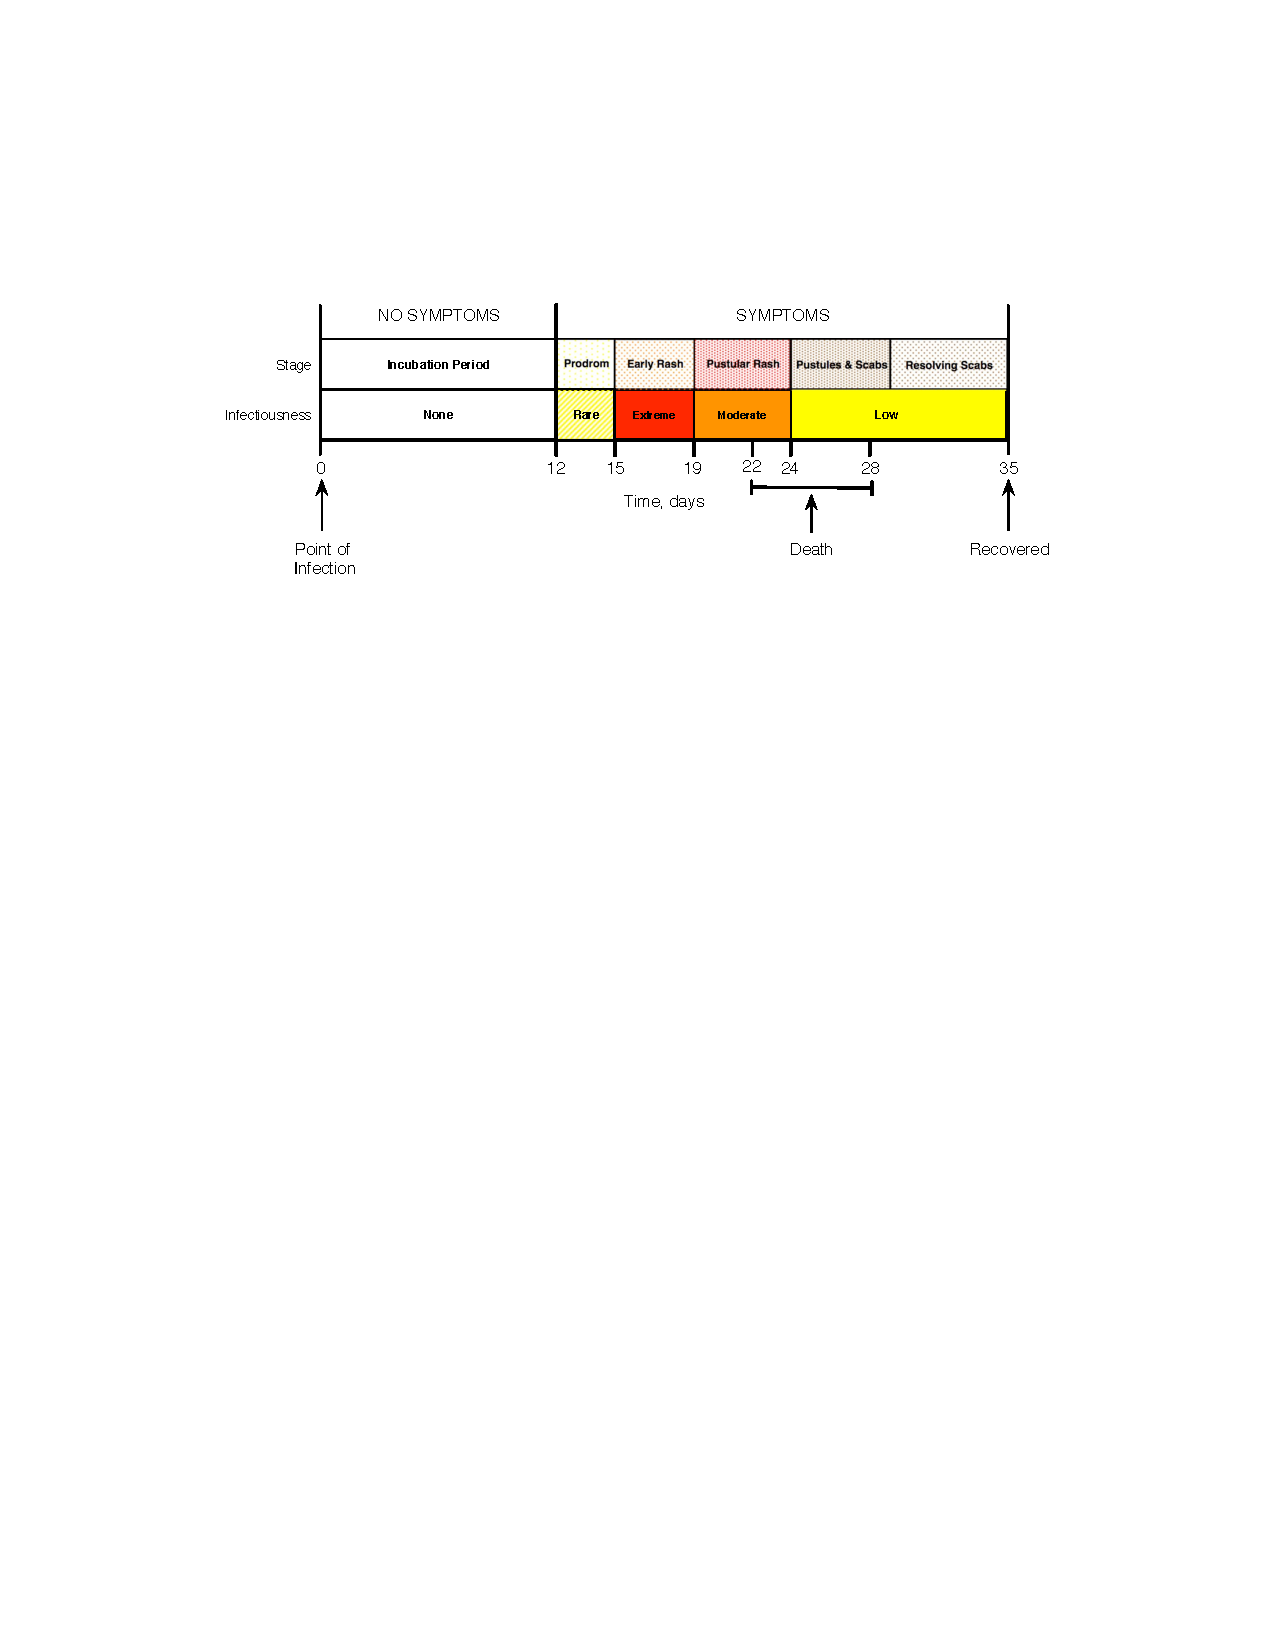
\includegraphics{smpxnathist_p82.pdf}
}
\end{center}
\caption{The natural history of smallpox infection. The prodrom stage begins with fever but the patient is very rarely contagious. Early rash is the most contagious stage, when the rash develops and transforms into bumps. During the pustular rash stage bumps become pustules, which then turn into scabs during the pustules and scabs stage and fall off during the resolving scabs stage. The infected person is contagious until the last scab falls off.  (\emph{This is Figure 3.4 from page 82 of Olga Krylova's 2011 McMaster University PhD thesis.})}
\label{F:smpxnathist}
\end{figure}
%
}

%%\bibliographystyle{vancouver}
%%\bibliography{4mba4_2018}

\newcommand{\BeautifulSolution}{{\color{blue}\begin{proof}{\color{magenta}\dots beautifully clear and concise text to be inserted here\dots}\end{proof}}}


\usepackage{fancyhdr,lastpage}
\pagestyle{fancy}
\fancyhf{} 
\lfoot{}
\cfoot{{\small\bfseries Page \thepage\ of \pageref{LastPage}}}
\rfoot{}
\renewcommand\headrulewidth{0pt}
\IfFileExists{upquote.sty}{\usepackage{upquote}}{}
\begin{document}

\begin{center}
{\bf Mathematics 4MB3/6MB3 Mathematical Biology\\
\smallskip
2016 ASSIGNMENT \textcolor{blue}{4}}\\
\medskip
\underline{\emph{Group Name}}: \texttt{{\color{blue}The Four Humours}}\\
\medskip
\underline{\emph{Group Members}}: {\color{blue}Claudia Tugulun, Roger Zhang, Alexei Kuzmin, Alexandra Bushby}
\end{center}

\bigskip
\noindent


\bigskip

\section{Time Series analysis of Recurrent Epidemics}

\begin{enumerate}[(a)]

\item 



\begin{enumerate}[(i)]

\item 


\begin{knitrout}
\definecolor{shadecolor}{rgb}{0.969, 0.969, 0.969}\color{fgcolor}\begin{kframe}
\begin{alltt}
\hlstd{londona} \hlkwb{<-} \hlkwd{read.csv}\hlstd{(}\hlstr{"meas_uk__lon_1944-94_wk.csv"}\hlstd{)}
\hlstd{liverpoola} \hlkwb{<-} \hlkwd{read.csv}\hlstd{(}\hlstr{"meas_uk__lpl_1944-94_wk.csv"}\hlstd{)}

\hlstd{londonb} \hlkwb{<-} \hlstd{londona[}\hlopt{-}\hlkwd{c}\hlstd{(}\hlnum{1}\hlstd{,}\hlnum{2}\hlstd{,}\hlnum{3}\hlstd{,}\hlnum{4}\hlstd{,}\hlnum{5}\hlstd{,}\hlnum{6}\hlstd{,}\hlnum{7}\hlstd{,}\hlnum{8}\hlstd{,}\hlnum{9}\hlstd{),]} \hlcom{##cleaning out not needed data}
\hlstd{liverpoolb} \hlkwb{<-} \hlstd{liverpoola[}\hlopt{-}\hlkwd{c}\hlstd{(}\hlnum{1}\hlstd{,}\hlnum{2}\hlstd{,}\hlnum{3}\hlstd{,}\hlnum{4}\hlstd{,}\hlnum{5}\hlstd{,}\hlnum{6}\hlstd{,}\hlnum{7}\hlstd{,}\hlnum{8}\hlstd{,}\hlnum{9}\hlstd{),]} \hlcom{##cleaning out not needed data}

\hlstd{read.ymdc} \hlkwb{<-} \hlkwa{function}\hlstd{(}\hlkwc{dat}\hlstd{)\{}
  \hlstd{year} \hlkwb{<-} \hlstd{dat[}\hlkwd{seq}\hlstd{(}\hlnum{1}\hlstd{,}\hlkwd{length}\hlstd{(dat),}\hlnum{4}\hlstd{)]}
  \hlstd{month} \hlkwb{<-}\hlstd{dat[}\hlkwd{seq}\hlstd{(}\hlnum{2}\hlstd{,}\hlkwd{length}\hlstd{(dat),}\hlnum{4}\hlstd{)]}
  \hlstd{day} \hlkwb{<-}\hlstd{dat[}\hlkwd{seq}\hlstd{(}\hlnum{3}\hlstd{,}\hlkwd{length}\hlstd{(dat),}\hlnum{4}\hlstd{)]}
  \hlstd{date}\hlkwb{<-}\hlkwd{as.Date}\hlstd{(}\hlkwd{paste}\hlstd{(year, month, day,} \hlkwc{sep} \hlstd{=} \hlstr{"."}\hlstd{),} \hlkwc{format} \hlstd{=} \hlstr{"%Y.%m.%d"}\hlstd{)}
  \hlstd{count} \hlkwb{<-}\hlstd{dat[}\hlkwd{seq}\hlstd{(}\hlnum{4}\hlstd{,}\hlkwd{length}\hlstd{(dat),}\hlnum{4}\hlstd{)]}
  \hlstd{count} \hlkwb{<-} \hlkwd{as.numeric}\hlstd{(}\hlkwd{as.character}\hlstd{(count))}
  \hlstd{week} \hlkwb{<-} \hlkwd{as.numeric}\hlstd{((date} \hlopt{-} \hlstd{date[}\hlnum{1}\hlstd{])}\hlopt{/}\hlnum{7}\hlstd{)}
  \hlstd{l} \hlkwb{<-} \hlkwd{list}\hlstd{(date, count, week)}
  \hlstd{L} \hlkwb{<-} \hlkwd{data.frame}\hlstd{(l)}
  \hlkwd{names}\hlstd{(L)} \hlkwb{<-}\hlkwd{c}\hlstd{(}\hlstr{"Date"}\hlstd{,} \hlstr{"Counts"}\hlstd{,} \hlstr{"Week"}\hlstd{)}
  \hlkwd{return}\hlstd{(L)}
\hlstd{\}}

\hlstd{London} \hlkwb{<-} \hlkwd{read.ymdc}\hlstd{(londonb)}
\hlstd{Liverpool} \hlkwb{<-}\hlkwd{read.ymdc}\hlstd{(liverpoolb)}
\end{alltt}
\end{kframe}
\end{knitrout}

\item 

\begin{knitrout}
\definecolor{shadecolor}{rgb}{0.969, 0.969, 0.969}\color{fgcolor}\begin{kframe}
\begin{alltt}
\hlkwd{par}\hlstd{(}\hlkwc{mfrow} \hlstd{=} \hlkwd{c}\hlstd{(}\hlnum{2}\hlstd{,}\hlnum{1}\hlstd{))}
\hlstd{m.average} \hlkwb{<-} \hlkwa{function}\hlstd{(}\hlkwc{dat}\hlstd{,}\hlkwc{n}\hlstd{)\{}\hlkwd{filter}\hlstd{(dat[,}\hlnum{2}\hlstd{],}\hlkwd{rep}\hlstd{(}\hlnum{1}\hlopt{/}\hlstd{(}\hlnum{2}\hlopt{*}\hlstd{n}\hlopt{+}\hlnum{1}\hlstd{),n),} \hlkwc{sides}\hlstd{=}\hlnum{2}\hlstd{)\}}

\hlstd{time.plot}\hlkwb{<-}\hlkwa{function}\hlstd{(}\hlkwc{dat}\hlstd{,}\hlkwc{add}\hlstd{=}\hlnum{FALSE}\hlstd{,} \hlkwc{n}\hlstd{=}\hlnum{20}\hlstd{,} \hlkwc{linetype} \hlstd{=} \hlstr{"l"}\hlstd{,} \hlkwc{colour} \hlstd{=} \hlstr{"red"}\hlstd{,}
                    \hlkwc{maint}\hlstd{)\{}
  \hlkwa{if}\hlstd{(add} \hlopt{==} \hlnum{TRUE}\hlstd{)\{}
    \hlstd{X}\hlkwb{<-}\hlkwd{plot}\hlstd{(dat}\hlopt{$}\hlstd{Week, dat}\hlopt{$}\hlstd{Counts,} \hlkwc{type}\hlstd{= linetype,} \hlkwc{xlab} \hlstd{=} \hlstr{"Time (Weeks)"}\hlstd{,}
            \hlkwc{ylab} \hlstd{=} \hlstr{"Cases of Measles"}\hlstd{,} \hlkwc{main} \hlstd{= maint)}
    \hlstd{lin} \hlkwb{<-} \hlkwd{lines}\hlstd{(}\hlkwd{m.average}\hlstd{(dat,n),} \hlkwc{col} \hlstd{= colour)}
  \hlstd{\}}
  \hlkwa{if}\hlstd{(add} \hlopt{==} \hlnum{FALSE}\hlstd{)\{}
    \hlstd{X}\hlkwb{<-}\hlkwd{plot}\hlstd{(dat}\hlopt{$}\hlstd{Week, dat}\hlopt{$}\hlstd{Counts,} \hlkwc{type} \hlstd{= linetype,} \hlkwc{xlab} \hlstd{=} \hlstr{"Time (Weeks)"}\hlstd{,}
            \hlkwc{ylab} \hlstd{=} \hlstr{"Cases of Measles"}\hlstd{,} \hlkwc{main} \hlstd{= maint)}
  \hlstd{\}}
\hlstd{\}}

\hlkwd{time.plot}\hlstd{(London,} \hlkwc{add} \hlstd{=} \hlnum{TRUE}\hlstd{,} \hlkwc{n} \hlstd{=} \hlnum{10}\hlstd{,} \hlkwc{col} \hlstd{=} \hlstr{"red"}\hlstd{,} \hlkwc{maint} \hlstd{=} \hlstr{"London"}\hlstd{)}
\hlkwd{time.plot}\hlstd{(Liverpool,} \hlkwc{add}\hlstd{=}\hlnum{TRUE}\hlstd{,} \hlkwc{n}\hlstd{=}\hlnum{10}\hlstd{,} \hlkwc{col} \hlstd{=} \hlstr{"red"}\hlstd{,} \hlkwc{maint} \hlstd{=} \hlstr{"Liverpool"}\hlstd{)}
\end{alltt}
\end{kframe}
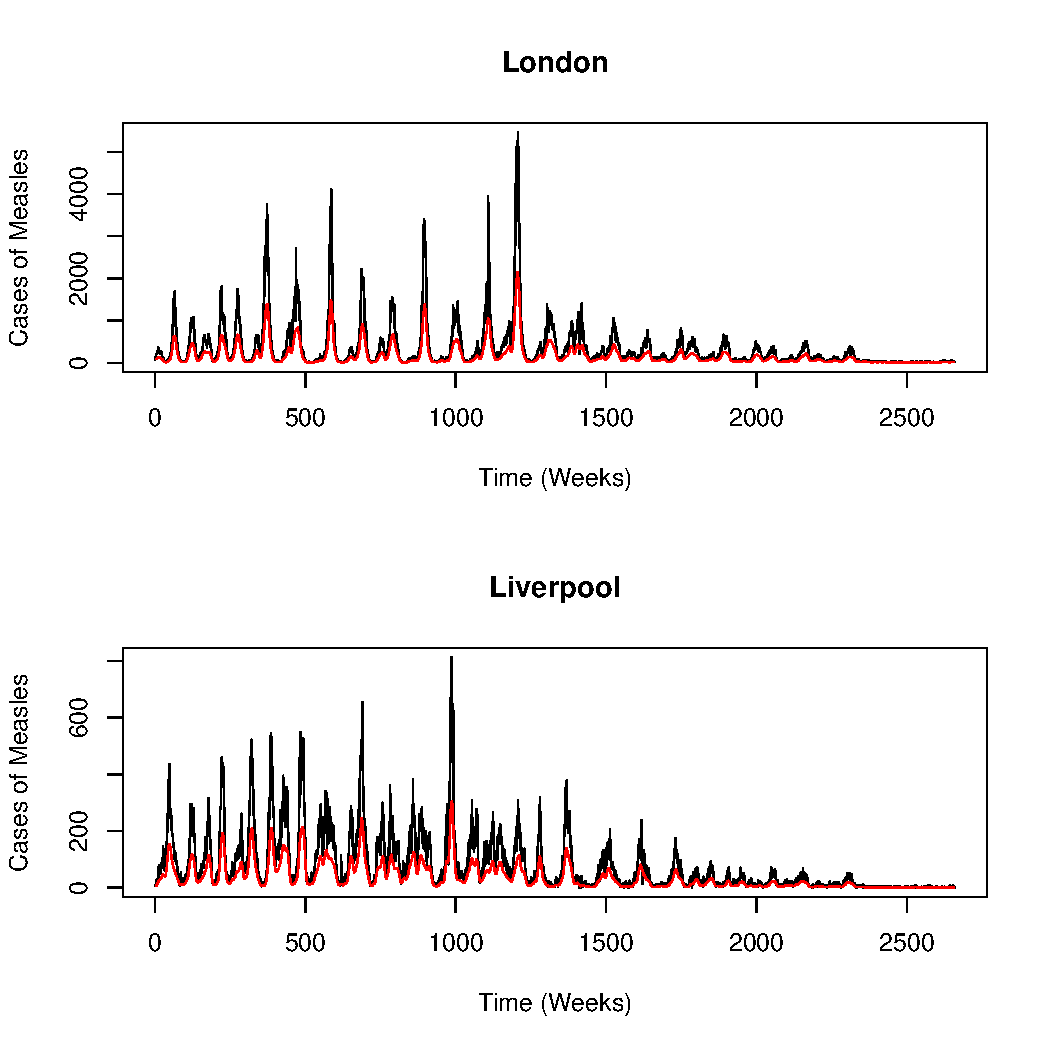
\includegraphics[width=\maxwidth]{figure/unnamed-chunk-2-1} 

\end{knitrout}


\item 
\begin{knitrout}
\definecolor{shadecolor}{rgb}{0.969, 0.969, 0.969}\color{fgcolor}\begin{kframe}
\begin{alltt}
\hlstd{periodogram}\hlkwb{<-}\hlkwa{function}\hlstd{(}\hlkwc{dat}\hlstd{,} \hlkwc{timemin} \hlstd{=} \hlnum{0}\hlstd{,} \hlkwc{timemax} \hlstd{=} \hlnum{2660}\hlstd{,} \hlkwc{linetype} \hlstd{=} \hlstr{"l"}\hlstd{,}
                      \hlkwc{colour} \hlstd{=} \hlstr{"black"}\hlstd{,} \hlkwc{maint}\hlstd{)\{}
  \hlstd{Uptodate} \hlkwb{<-} \hlstd{dat[dat}\hlopt{$}\hlstd{Week} \hlopt{>=} \hlstd{timemin} \hlopt{&} \hlstd{dat}\hlopt{$}\hlstd{Week} \hlopt{<=} \hlstd{timemax , ]}
  \hlstd{s}\hlkwb{<-}\hlkwd{spectrum}\hlstd{(Uptodate}\hlopt{$}\hlstd{Counts,} \hlkwc{plot}\hlstd{=}\hlnum{FALSE}\hlstd{)}
  \hlstd{per} \hlkwb{<-}  \hlnum{1}\hlopt{/}\hlstd{(s}\hlopt{$}\hlstd{freq}\hlopt{*}\hlnum{52}\hlstd{)}
  \hlstd{spec} \hlkwb{<-} \hlstd{s}\hlopt{$}\hlstd{spec}\hlopt{/}\hlkwd{max}\hlstd{(s}\hlopt{$}\hlstd{spec)}
  \hlkwd{plot}\hlstd{(per, spec,} \hlkwc{type} \hlstd{= linetype,} \hlkwc{xlab} \hlstd{=} \hlstr{"Period (Years)"}\hlstd{,}
       \hlkwc{ylab} \hlstd{=} \hlstr{"Power Spectrum"}\hlstd{,} \hlkwc{xlim} \hlstd{=} \hlkwd{c}\hlstd{(}\hlnum{0}\hlstd{,}\hlnum{5}\hlstd{),} \hlkwc{col} \hlstd{= colour,} \hlkwc{main} \hlstd{= maint)}
\hlstd{\}}
\end{alltt}
\end{kframe}
\end{knitrout}

\end{enumerate}

\item

\begin{knitrout}
\definecolor{shadecolor}{rgb}{0.969, 0.969, 0.969}\color{fgcolor}\begin{kframe}
\begin{alltt}
\hlkwd{par}\hlstd{(}\hlkwc{mfrow} \hlstd{=} \hlkwd{c}\hlstd{(}\hlnum{4}\hlstd{,}\hlnum{2}\hlstd{))}

\hlkwd{periodogram}\hlstd{(London,} \hlkwc{timemax} \hlstd{=} \hlnum{400}\hlstd{,} \hlkwc{maint} \hlstd{=} \hlstr{"London (1944 - 1951)"}\hlstd{)}
\hlkwd{periodogram}\hlstd{(Liverpool,} \hlkwc{timemax} \hlstd{=} \hlnum{400}\hlstd{,} \hlkwc{maint} \hlstd{=} \hlstr{"Liverpool (1944-1951)"}\hlstd{)}
\hlkwd{periodogram}\hlstd{(London,} \hlkwc{timemin} \hlstd{=} \hlnum{400}\hlstd{,} \hlkwc{timemax} \hlstd{=} \hlnum{1250}\hlstd{,}
            \hlkwc{maint} \hlstd{=} \hlstr{"London (1951-1967)"}\hlstd{)}
\hlkwd{periodogram}\hlstd{(Liverpool,} \hlkwc{timemin} \hlstd{=} \hlnum{400}\hlstd{,} \hlkwc{timemax} \hlstd{=} \hlnum{1250}\hlstd{,}
            \hlkwc{maint} \hlstd{=} \hlstr{"Liverpool (1951-1967)"}\hlstd{)}
\hlkwd{periodogram}\hlstd{(London,} \hlkwc{timemin} \hlstd{=} \hlnum{1250}\hlstd{,} \hlkwc{timemax} \hlstd{=} \hlnum{2400}\hlstd{,}
            \hlkwc{maint} \hlstd{=} \hlstr{"London (1967 - 1990)"}\hlstd{)}
\hlkwd{periodogram}\hlstd{(Liverpool,} \hlkwc{timemin} \hlstd{=} \hlnum{1250}\hlstd{,} \hlkwc{timemax} \hlstd{=} \hlnum{2400}\hlstd{,}
            \hlkwc{maint} \hlstd{=} \hlstr{"Liverpool (1967 - 1990)"}\hlstd{)}
\hlkwd{periodogram}\hlstd{(London,} \hlkwc{timemin} \hlstd{=} \hlnum{2400}\hlstd{,} \hlkwc{maint} \hlstd{=} \hlstr{"London (1990-1994)"}\hlstd{)}
\hlkwd{periodogram}\hlstd{(Liverpool,} \hlkwc{timemin} \hlstd{=} \hlnum{2400}\hlstd{,} \hlkwc{maint} \hlstd{=} \hlstr{"Liverpool (1990-1994)"}\hlstd{)}
\end{alltt}
\end{kframe}
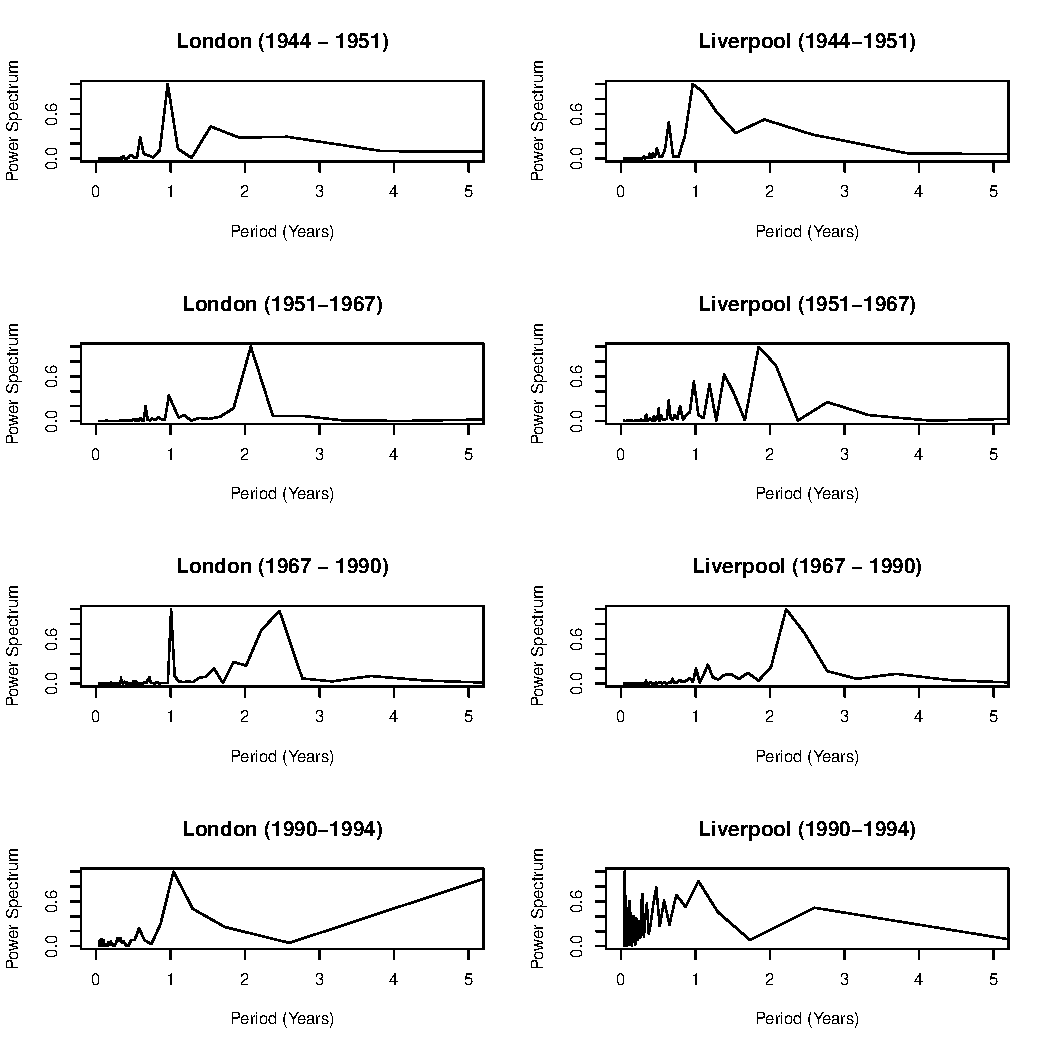
\includegraphics[width=\maxwidth]{figure/unnamed-chunk-4-1} 

\end{knitrout}

The above periodograms were chosen because that's when the data appeared to change on the timeplot. London's periodogram and Liverpool's periodogram are very different. London seems to almost always have a period of 1 year, as well as an additional period, such as 2 or 2.5 years. Liverpool has a much more interesting and vast plot, but also shows some similarities to London's periodogram. For example, Liverpool and London both have high power at 1 year from 1944-1951, high power at 2 years from 1951-1967 high power at 2.5 years from 1967-1990 and then high power back at 1 year from 1990-1994. What is interesting about the periodogram is Liverpool from 1990-1994. It seems as though there is a lot of power at certain intervals between 0 and 1 year. It would be very useful to use mathematical modelling to determine the reason for this change in periods and, in addition, to understand why the period being 1 year almost always has a lot of power.

\end{enumerate}

\section{Stochastic Epidemic Simulations}

\begin{enumerate}[(a)]

\item

\begin{knitrout}
\definecolor{shadecolor}{rgb}{0.969, 0.969, 0.969}\color{fgcolor}\begin{kframe}
\begin{alltt}
\hlstd{SI.gillespie} \hlkwb{<-} \hlkwa{function}\hlstd{(}\hlkwc{beta}\hlstd{,} \hlkwc{N}\hlstd{,} \hlkwc{I0}\hlstd{,} \hlkwc{tmax}\hlstd{)\{}
  \hlstd{t0} \hlkwb{<-} \hlnum{0}
  \hlstd{times} \hlkwb{=}\hlstd{(t0}\hlopt{:}\hlstd{tmax)}
  \hlstd{x} \hlkwb{<-}\hlkwd{c}\hlstd{(}\hlkwc{S}\hlstd{=N}\hlopt{-}\hlstd{I0,} \hlkwc{I}\hlstd{=I0,} \hlkwc{t}\hlstd{=t0)}

  \hlstd{res} \hlkwb{<-} \hlkwd{matrix}\hlstd{(}\hlkwc{nrow}\hlstd{=}\hlkwd{length}\hlstd{(t0}\hlopt{:}\hlstd{tmax),}\hlkwc{ncol}\hlstd{=}\hlkwd{length}\hlstd{(x),}
                \hlkwc{dimnames} \hlstd{=} \hlkwd{list}\hlstd{(times,}\hlkwd{names}\hlstd{(x)))} \hlcom{#matrix to store values}

  \hlkwa{for} \hlstd{(i} \hlkwa{in} \hlnum{1}\hlopt{:}\hlstd{(tmax}\hlopt{+}\hlnum{1}\hlstd{))\{}
    \hlstd{res[i,]} \hlkwb{<-} \hlstd{x}
    \hlstd{rate} \hlkwb{<-} \hlkwd{with}\hlstd{(}\hlkwd{as.list}\hlstd{(x), beta}\hlopt{*}\hlstd{S}\hlopt{*}\hlstd{I)} \hlcom{## calculate current rate}
    \hlkwa{if}\hlstd{(rate}\hlopt{<=}\hlnum{0}\hlstd{)} \hlkwa{break} \hlcom{#rate != 0; t_next would return NaN}
    \hlstd{t_next} \hlkwb{<-} \hlkwd{rexp}\hlstd{(}\hlnum{1}\hlstd{,rate)}  \hlcom{#time to next event}
    \hlstd{t0} \hlkwb{<-} \hlstd{t0} \hlopt{+} \hlstd{t_next} \hlcom{# update time}
    \hlstd{x} \hlkwb{<-} \hlstd{x}\hlopt{+}\hlkwd{c}\hlstd{(}\hlopt{-}\hlnum{1}\hlopt{*}\hlstd{rate}\hlopt{*}\hlstd{t_next,} \hlnum{1}\hlopt{*}\hlstd{rate}\hlopt{*}\hlstd{t_next, t0)} \hlcom{#updates x <- c(S, I, t)}
    \hlkwa{if}\hlstd{(x[}\hlnum{1}\hlstd{]}\hlopt{<}\hlnum{0}\hlstd{)} \hlcom{#if S is for some reason negative, }
      \hlcom{#change it to its previous positive}
      \hlstd{x} \hlkwb{<-} \hlstd{res[i,]}
  \hlstd{\}}
  \hlkwd{cbind}\hlstd{(res[,}\hlnum{3}\hlstd{],res[,}\hlnum{2}\hlstd{])} \hlcom{#returns cbind(t, I)}
\hlstd{\}}
\end{alltt}
\end{kframe}
\end{knitrout}


\item 

\begin{knitrout}
\definecolor{shadecolor}{rgb}{0.969, 0.969, 0.969}\color{fgcolor}\begin{kframe}
\begin{alltt}
\hlkwd{par}\hlstd{(}\hlkwc{mfrow} \hlstd{=} \hlkwd{c}\hlstd{(}\hlnum{2}\hlstd{,}\hlnum{2}\hlstd{))}

\hlcom{## N=32}
\hlkwd{plot}\hlstd{(}\hlnum{0}\hlstd{,}\hlnum{0}\hlstd{,}\hlkwc{xlim}\hlstd{=}\hlkwd{c}\hlstd{(}\hlnum{0}\hlstd{,}\hlnum{10}\hlstd{),}\hlkwc{ylim}\hlstd{=}\hlkwd{c}\hlstd{(}\hlnum{0}\hlstd{,}\hlnum{32}\hlstd{),}
     \hlkwc{type}\hlstd{=}\hlstr{"n"}\hlstd{,}\hlkwc{xlab}\hlstd{=}\hlstr{"Time (t)"}\hlstd{,}\hlkwc{ylab}\hlstd{=}\hlstr{"Prevalence (I)"}\hlstd{,}\hlkwc{main} \hlstd{=} \hlstr{"N = 32"}\hlstd{,} \hlkwc{las}\hlstd{=}\hlnum{1}\hlstd{)}
\hlkwa{for}\hlstd{(i} \hlkwa{in} \hlnum{1}\hlopt{:}\hlnum{30}\hlstd{)\{}
  \hlstd{G.SI} \hlkwb{<-} \hlkwd{SI.gillespie}\hlstd{(}\hlkwc{beta}\hlstd{=}\hlnum{1}\hlstd{,} \hlkwc{N}\hlstd{=}\hlnum{32}\hlstd{,} \hlkwc{I0}\hlstd{=}\hlnum{1}\hlstd{,} \hlkwc{tmax}\hlstd{=}\hlnum{80}\hlstd{)}
  \hlkwd{lines}\hlstd{(G.SI,} \hlkwc{col}\hlstd{=i)}
\hlstd{\}}
\hlstd{N} \hlkwb{<-} \hlnum{32}
\hlstd{beta} \hlkwb{<-} \hlnum{1}
\hlstd{I0} \hlkwb{<-} \hlnum{1}
\hlstd{It} \hlkwb{<-} \hlstd{I0}\hlopt{*}\hlkwd{exp}\hlstd{(N}\hlopt{*}\hlstd{beta}\hlopt{*}\hlstd{G.SI[,}\hlnum{1}\hlstd{])}\hlopt{/}\hlstd{(}\hlnum{1}\hlopt{+}\hlstd{(I0}\hlopt{/}\hlstd{N)}\hlopt{*}\hlstd{(}\hlkwd{exp}\hlstd{(N}\hlopt{*}\hlstd{beta}\hlopt{*}\hlstd{G.SI[,}\hlnum{1}\hlstd{])}\hlopt{-}\hlnum{1}\hlstd{))}
\hlkwd{lines}\hlstd{(G.SI[,}\hlnum{1}\hlstd{],It,}\hlkwc{lwd}\hlstd{=}\hlnum{3}\hlstd{)}

\hlcom{## N=100}
\hlkwd{plot}\hlstd{(}\hlnum{0}\hlstd{,}\hlnum{0}\hlstd{,}\hlkwc{xlim}\hlstd{=}\hlkwd{c}\hlstd{(}\hlnum{0}\hlstd{,}\hlnum{10}\hlstd{),}\hlkwc{ylim}\hlstd{=}\hlkwd{c}\hlstd{(}\hlnum{0}\hlstd{,}\hlnum{100}\hlstd{),}
     \hlkwc{type}\hlstd{=}\hlstr{"n"}\hlstd{,}\hlkwc{xlab}\hlstd{=}\hlstr{"Time (t)"}\hlstd{,}\hlkwc{ylab}\hlstd{=}\hlstr{"Prevalence (I)"}\hlstd{,}\hlkwc{las}\hlstd{=}\hlnum{1}\hlstd{,} \hlkwc{main} \hlstd{=} \hlstr{"N = 100"}\hlstd{)}
\hlkwa{for}\hlstd{(i} \hlkwa{in} \hlnum{1}\hlopt{:}\hlnum{30}\hlstd{)\{}
  \hlstd{G.SI} \hlkwb{<-} \hlkwd{SI.gillespie}\hlstd{(}\hlkwc{beta}\hlstd{=}\hlnum{1}\hlstd{,} \hlkwc{N}\hlstd{=}\hlnum{100}\hlstd{,} \hlkwc{I0}\hlstd{=}\hlnum{1}\hlstd{,} \hlkwc{tmax}\hlstd{=}\hlnum{300}\hlstd{)}
  \hlkwd{lines}\hlstd{(G.SI,} \hlkwc{col}\hlstd{=i)}
\hlstd{\}}
\hlstd{N} \hlkwb{<-} \hlnum{100}
\hlstd{G.SI} \hlkwb{<-} \hlkwd{SI.gillespie}\hlstd{(}\hlkwc{beta}\hlstd{=}\hlnum{1}\hlstd{,} \hlkwc{N}\hlstd{=}\hlnum{100}\hlstd{,} \hlkwc{I0}\hlstd{=}\hlnum{1}\hlstd{,} \hlkwc{tmax}\hlstd{=}\hlnum{80}\hlstd{)}
\hlstd{It} \hlkwb{<-} \hlstd{I0}\hlopt{*}\hlkwd{exp}\hlstd{(N}\hlopt{*}\hlstd{beta}\hlopt{*}\hlstd{G.SI[,}\hlnum{1}\hlstd{])}\hlopt{/}\hlstd{(}\hlnum{1}\hlopt{+}\hlstd{(I0}\hlopt{/}\hlstd{N)}\hlopt{*}\hlstd{(}\hlkwd{exp}\hlstd{(N}\hlopt{*}\hlstd{beta}\hlopt{*}\hlstd{G.SI[,}\hlnum{1}\hlstd{])}\hlopt{-}\hlnum{1}\hlstd{))}
\hlkwd{lines}\hlstd{(G.SI[,}\hlnum{1}\hlstd{],It,}\hlkwc{lwd}\hlstd{=}\hlnum{3}\hlstd{)}

\hlcom{## N=1000}
\hlkwd{plot}\hlstd{(}\hlnum{0}\hlstd{,}\hlnum{0}\hlstd{,}\hlkwc{xlim}\hlstd{=}\hlkwd{c}\hlstd{(}\hlnum{0}\hlstd{,}\hlnum{10}\hlstd{),}\hlkwc{ylim}\hlstd{=}\hlkwd{c}\hlstd{(}\hlnum{0}\hlstd{,}\hlnum{1000}\hlstd{),}
     \hlkwc{type}\hlstd{=}\hlstr{"n"}\hlstd{,}\hlkwc{xlab}\hlstd{=}\hlstr{"Time (t)"}\hlstd{,}\hlkwc{ylab}\hlstd{=}\hlstr{"Prevalence (I)"}\hlstd{,}\hlkwc{las}\hlstd{=}\hlnum{1}\hlstd{,} \hlkwc{main} \hlstd{=} \hlstr{"N = 1000"}\hlstd{)}
\hlkwa{for}\hlstd{(i} \hlkwa{in} \hlnum{1}\hlopt{:}\hlnum{30}\hlstd{)\{}
  \hlstd{G.SI} \hlkwb{<-} \hlkwd{SI.gillespie}\hlstd{(}\hlkwc{beta}\hlstd{=}\hlnum{1}\hlstd{,} \hlkwc{N}\hlstd{=}\hlnum{1000}\hlstd{,} \hlkwc{I0}\hlstd{=}\hlnum{1}\hlstd{,} \hlkwc{tmax}\hlstd{=}\hlnum{1000}\hlstd{)}
  \hlkwd{lines}\hlstd{(G.SI,} \hlkwc{col}\hlstd{=i)}
\hlstd{\}}
\hlstd{N} \hlkwb{<-} \hlnum{1000}
\hlstd{It} \hlkwb{<-} \hlstd{I0}\hlopt{*}\hlkwd{exp}\hlstd{(N}\hlopt{*}\hlstd{beta}\hlopt{*}\hlstd{G.SI[,}\hlnum{1}\hlstd{])}\hlopt{/}\hlstd{(}\hlnum{1}\hlopt{+}\hlstd{(I0}\hlopt{/}\hlstd{N)}\hlopt{*}\hlstd{(}\hlkwd{exp}\hlstd{(N}\hlopt{*}\hlstd{beta}\hlopt{*}\hlstd{G.SI[,}\hlnum{1}\hlstd{])}\hlopt{-}\hlnum{1}\hlstd{))}
\hlkwd{lines}\hlstd{(G.SI[,}\hlnum{1}\hlstd{],It,}\hlkwc{lwd}\hlstd{=}\hlnum{3}\hlstd{)}

\hlcom{## N=10,000}
\hlkwd{plot}\hlstd{(}\hlnum{0}\hlstd{,}\hlnum{0}\hlstd{,}\hlkwc{xlim}\hlstd{=}\hlkwd{c}\hlstd{(}\hlnum{0}\hlstd{,}\hlnum{10}\hlstd{),}\hlkwc{ylim}\hlstd{=}\hlkwd{c}\hlstd{(}\hlnum{0}\hlstd{,}\hlnum{10000}\hlstd{),}
     \hlkwc{type}\hlstd{=}\hlstr{"n"}\hlstd{,}\hlkwc{xlab}\hlstd{=}\hlstr{"Time (t)"}\hlstd{,}\hlkwc{ylab}\hlstd{=}\hlstr{"Prevalence (I)"}\hlstd{,}\hlkwc{las}\hlstd{=}\hlnum{1}\hlstd{,} \hlkwc{main} \hlstd{=} \hlstr{"N = 10,000"}\hlstd{)}
\hlkwa{for}\hlstd{(i} \hlkwa{in} \hlnum{1}\hlopt{:}\hlnum{30}\hlstd{)\{}
  \hlstd{G.SI} \hlkwb{<-} \hlkwd{SI.gillespie}\hlstd{(}\hlkwc{beta}\hlstd{=}\hlnum{1}\hlstd{,} \hlkwc{N}\hlstd{=}\hlnum{10000}\hlstd{,} \hlkwc{I0}\hlstd{=}\hlnum{1}\hlstd{,} \hlkwc{tmax}\hlstd{=}\hlnum{10000}\hlstd{)}
  \hlkwd{lines}\hlstd{(G.SI,} \hlkwc{col}\hlstd{=i)}
\hlstd{\}}
\hlstd{N} \hlkwb{<-} \hlnum{10000}
\hlstd{It} \hlkwb{<-} \hlstd{I0}\hlopt{*}\hlkwd{exp}\hlstd{(N}\hlopt{*}\hlstd{beta}\hlopt{*}\hlstd{G.SI[,}\hlnum{1}\hlstd{])}\hlopt{/}\hlstd{(}\hlnum{1}\hlopt{+}\hlstd{(I0}\hlopt{/}\hlstd{N)}\hlopt{*}\hlstd{(}\hlkwd{exp}\hlstd{(N}\hlopt{*}\hlstd{beta}\hlopt{*}\hlstd{G.SI[,}\hlnum{1}\hlstd{])}\hlopt{-}\hlnum{1}\hlstd{))}
\hlkwd{lines}\hlstd{(G.SI[,}\hlnum{1}\hlstd{],It,}\hlkwc{lwd}\hlstd{=}\hlnum{3}\hlstd{)}
\end{alltt}
\end{kframe}
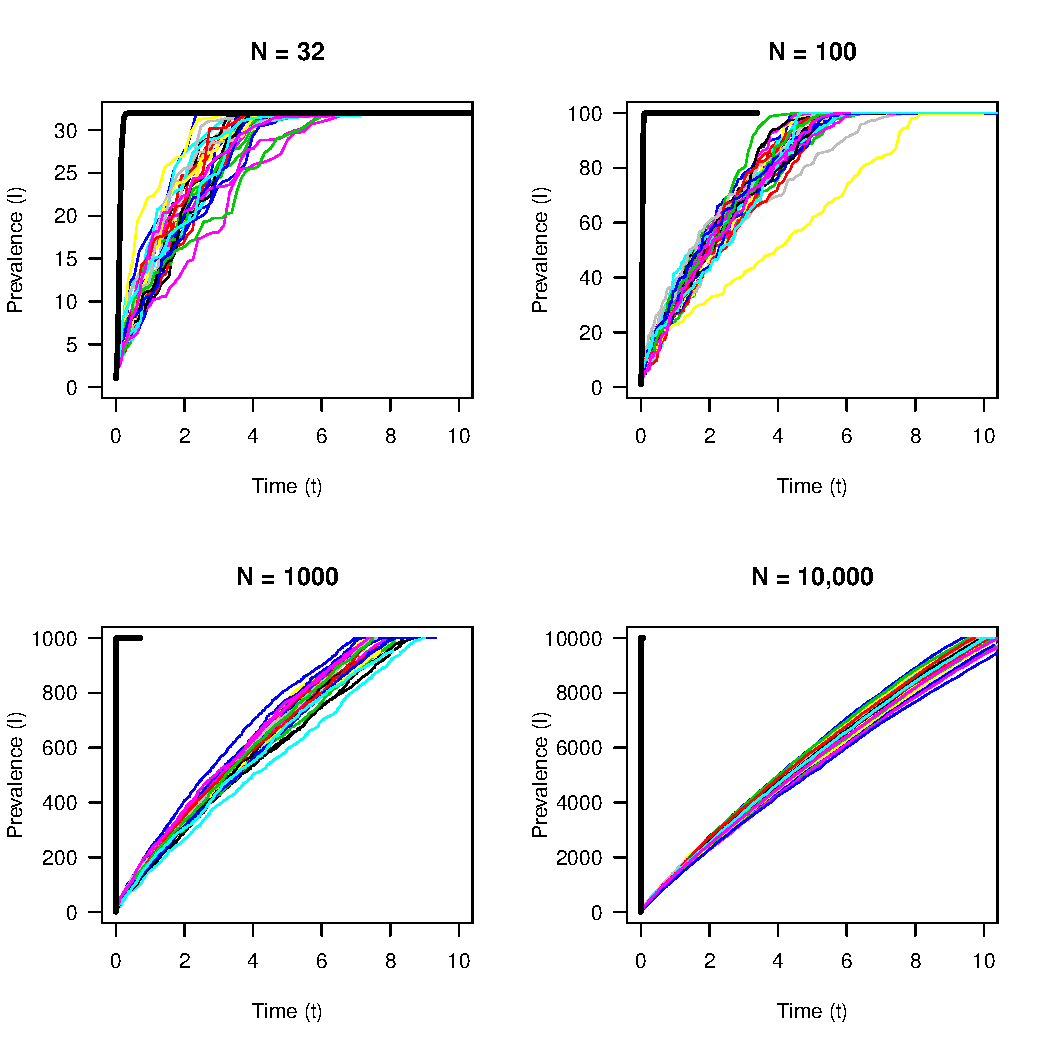
\includegraphics[width=\maxwidth]{figure/unnamed-chunk-6-1} 

\end{knitrout}


\end{enumerate}

\section{$\R_0$ for smallpox}

\begin{enumerate}[(a)]

\item

$I_i$ corresponds to the infectious state an individual is in. $\mu$ is the per capita rate of births and deaths and $\beta_i$ is the transmission rate, which depends on which stage of the infection an individual is in. When $i=R$, we have rare infectiousness. When $i=E$, we have extreme infectiousness. When $i=M$, we have moderate infectiousness. When $i=L$, we have low infectiousness. 
\begin{subequations}
\begin{align}
\frac{dS}{dt} &= \mu - S \mu - S (\beta_R I _R + \beta_E I _E + \beta_M I_M + \beta_L I_L) \\
\noalign{\vspace{8pt}}
\frac{dE}{dt} &= S (\beta_R I _R + \beta_E I _E + \beta_M I_M + \beta_L I_L) - \mu E - \frac{1}{12} E \\
\noalign{\vspace{8pt}}
\frac{dI_R}{dt} &= \frac{1}{12} E - \frac{1}{3} I_R - \mu I_R \\
\noalign{\vspace{8pt}}
\frac{dI_E}{dt} &= \frac{1}{3} I_R - \frac{1}{4} I_E - \mu I_E \\
\noalign{\vspace{8pt}}
\frac{dI_M}{dt} &= \frac{1}{4} I_E - \frac{1}{5} I_M - \mu I_M \\
\noalign{\vspace{8pt}}
\frac{dI_L}{dt} &= \frac{1}{5} I_M - \frac{1}{11} I_L - \mu I_L \\
\noalign{\vspace{8pt}}
\frac{dR}{dt} &= \frac{1}{11} I_L - \mu R
\end{align}
\end{subequations}

  \item

We have four stages of infections. 
Since each stage of infection results in secondary cases, each of the four stages must be considered individually and each corresponding $\R_0$ computed. The $\R_0$ of each stage is determined by the product of the corresponding transmission rate and average length of time an individual spends in that stage, which takes into account the probability of reaching and completing that particular stage of infection. The total $\R_0$ of the infectious disease is thus the sum of the reproductive numbers associated with each infected stage. The biological derivation of $\R_0$ is shown below.

\begin{multline}\label{eq:pareto mle2}
\R_0 = \beta_R \cdot \frac{\frac{1}{12}}{\frac{1}{12}+\mu}\cdot\frac{1}{\frac{1}{3}+\mu}+\beta_E \cdot \frac{\frac{1}{12}}{\frac{1}{12}+\mu}\cdot\frac{\frac{1}{3}}{\frac{1}{3}+\mu}\cdot\frac{1}{\frac{1}{4}+\mu}+\beta_M \cdot \frac{\frac{1}{12}}{\frac{1}{12}+\mu}\cdot\frac{\frac{1}{3}}{\frac{1}{3}+\mu}\cdot\frac{\frac{1}{4}}{\frac{1}{4}+\mu}\cdot\frac{1}{\frac{1}{5}+\mu} \\ +\beta_L \cdot \frac{\frac{1}{12}}{\frac{1}{12}+\mu}\cdot\frac{\frac{1}{3}}{\frac{1}{3}+\mu}\cdot\frac{\frac{1}{4}}{\frac{1}{4}+\mu}\cdot\frac{\frac{1}{5}}{\frac{1}{5}+\mu}\cdot\frac{1}{\frac{1}{11}+\mu}
\end{multline}
\begin{multline}\label{R01}
\R_0 =  \frac{3\beta_R}{(12 \mu + 1)(3 \mu + 1)} + \frac{4\beta_E}{(12 \mu + 1)(3 \mu + 1)  (4 \mu + 1)} +\frac{5\beta_M}{(12 \mu + 1)(3 \mu + 1)  (4 \mu + 1) (5 \mu + 1)} \\
+ \frac{11 \beta_L}{(12 \mu + 1)(3 \mu + 1)  (4 \mu + 1) (5 \mu + 1)(11\mu+1)}
\end{multline}


\item 
$ \mathcal{F}$ is the inflow of new infecteds and $F$ is the linearization at the DFE of $\mathcal{F}$.  $ \mathcal{V}$ is the outflow from infected individuals minus the inflow of non-new infecteds and $V$ is the linearization at the DFE of $\mathcal{V}$. 
\begin{align*}
\frac{d}{dt} \begin{pmatrix}
E \\
I_R \\
I_E \\
I_M \\
I_L
\end{pmatrix} &= \begin{pmatrix}
S (\beta_R I _R + \beta_E I _E + \beta_M I_M + \beta_L I_L) - \mu E - \frac{1}{12} E \\
\frac{1}{12} E - \frac{1}{3} I_R - \mu I_R\\
\frac{1}{3} I_R - \frac{1}{4} I_E - \mu I_E \\
\frac{1}{4} I_E - \frac{1}{5} I_M - \mu I_M \\
\frac{1}{5} I_M - \frac{1}{11} I_L - \mu I_L
\end{pmatrix} \\
\mathcal{F} &= \begin{pmatrix}
S (\beta_R I _R + \beta_E I _E + \beta_M I_M + \beta_L I_L) \\
0\\
0 \\
0 \\
0
\end{pmatrix} \\
F &= \begin{pmatrix}
0 & \beta_R & \beta_E & \beta_M & \beta_L \\
0 & 0 & 0 & 0 & 0\\
0 & 0 & 0 & 0 & 0\\
0 & 0 & 0 & 0 & 0\\
0 & 0 & 0 & 0 & 0
\end{pmatrix}  \\
\mathcal{V} &= \begin{pmatrix}
\mu E + \frac{1}{12} E \\
- \frac{1}{12} E + \frac{1}{3} I_R + \mu I_R\\
- \frac{1}{3} I_R + \frac{1}{4} I_E + \mu I_E \\
- \frac{1}{4} I_E + \frac{1}{5} I_M + \mu I_M \\
- \frac{1}{5} I_M + \frac{1}{11} I_L + \mu I_L
\end{pmatrix}  \\
V &= \begin{pmatrix}
\mu + \frac{1}{12} & 0 & 0 & 0 & 0\\
- \frac{1}{12} & \frac{1}{3} + \mu & 0 & 0 &0 \\
0 & - \frac{1}{3} & \frac{1}{4} + \mu & 0 & 0 \\
0 & 0 & - \frac{1}{4} & \frac{1}{5} + \mu & 0 \\
0 & 0 & 0 & - \frac{1}{5} & \frac{1}{11} + \mu
\end{pmatrix} \\
\end{align*}

According to WolframAlpha, $V^{-1}$ is:
\[
\begin{pmatrix}
\frac{12}{12\mu+1} & 0 & 0 & 0 & 0 \\
\frac{3}{(12\mu+1)(3\mu+1)} & \frac{3}{3\mu + 1} & 0 & 0&0 \\
\frac{4}{(12\mu+1)(3\mu+1)(4\mu+1)} & \frac{4}{(3\mu+1)(4\mu+1)} & \frac{4}{4 \mu + 1} & 0 & 0 \\
\frac{5}{(12\mu+1)(3\mu+1)(4\mu+1)(5\mu+1)} & \frac{5}{(3\mu+1)(4\mu+1)(5\mu+1)} & \frac{5}{(4\mu+1)(5\mu+1)}& \frac{5}{5 \mu + 1}& 0 \\
\frac{11}{(12\mu+1)(3\mu+1)(4\mu+1)(5\mu+1)(11\mu+1)}& \frac{11}{(3\mu+1)(4\mu+1)(5\mu+1)(11\mu+1)}& \frac{11}{(4\mu+1)(5\mu+1)(11\mu+1)} & \frac{11}{(5\mu+1)(11\mu+1)} & \frac{11}{11+\mu} 
\end{pmatrix}.
\]

The eigenvalues of $FV^{-1}$ can be found to be 0 or the following:
\begin{align*}
\lambda &= \frac{\beta_R(660 \mu^3 + 357 \mu^2 + 60 \mu + 3)+4\beta_E(55 \mu^2 + 16 \mu + 1)+5\beta_M(11+\mu) + 11 \beta_L}{(12 \mu + 1)(3 \mu + 1)  (4 \mu + 1) (5 \mu + 1)(11\mu+1)} \\
\lambda &= \frac{3\beta_R(4 \mu + 1) (5 \mu + 1)   (11 \mu + 1)+ 4\beta_E (5 \mu + 1)(11 \mu + 1) + 5\beta_M(11+\mu) + 11 \beta_L}{(12 \mu + 1)(3 \mu + 1)  (4 \mu + 1) (5 \mu + 1)(11\mu+1)}
\end{align*}

Because $\lambda = \rho(FV^{-1})$, $R_0$ is the following:
\begin{multline}\label{R02}
\R_0 = \frac{3\beta_R}{(12 \mu + 1)(3 \mu + 1)} + \frac{4\beta_E}{(12 \mu + 1)(3 \mu + 1)  (4 \mu + 1)} + \frac{5\beta_M}{(12 \mu + 1)(3 \mu + 1)  (4 \mu + 1) (5 \mu + 1)} \\ + \frac{11 \beta_L}{(12 \mu + 1)(3 \mu + 1)  (4 \mu + 1) (5 \mu + 1)(11\mu+1)}
\end{multline}

We can see that \eqref{R01} and \eqref{R02} agree with each other.

\item 
According to the CDC, the altered virus is characterized by the early rash stage lasting twice as long compared with the naturally circulating virus. That is, for the altered virus, the early rash stage is expected to last 8 days instead of 4 days. In practice, the value of $\R_0$ for the altered smallpox virus, $\R_0^A$, can be obtained by changing values of 4 to 8 in \eqref{R02}:

\begin{multline}\label{eq:R0_alt}
\R_0^A = \frac{3\beta_R}{(12 \mu + 1)(3 \mu + 1)} + \frac{8\beta_E}{(12 \mu + 1)(3 \mu + 1)  (8 \mu + 1)} + \frac{5\beta_M}{(12 \mu + 1)(3 \mu + 1)  (8 \mu + 1) (5 \mu + 1)} \\ + \frac{11 \beta_L}{(12 \mu + 1)(3 \mu + 1)  (8 \mu + 1) (5 \mu + 1)(11\mu+1)}
\end{multline}
Intuitively, we expect that $\R_0^A > \R_0$. As in part (b), $\R_0^A$ is composed of the sum of the reproductive numbers associated with each of the four infected stages. The reproductive number associated with the first stage (rare infectiousness) is unchanged for for the altered virus, i.e. $\R_0^A = \R_0$. Comparing equations \eqref{R02} and \eqref{eq:R0_alt}, we find the relationship between the reproductive number corresponding to the second stage (extreme infectiousness) for the altered and unaltered virus is $\R_0^A =2  \R_0 \frac{4 \mu + 1}{8 \mu + 1}$, where the multiplicative factor $\frac{4 \mu + 1}{8 \mu + 1}$ represents the probability of progressing through the second stage with the altered virus as a proportion of the probability of progressing through the second stage with the unaltered virus. For the final stages (moderate and low infectiousness), the relationship between the altered and unaltered reproductive numbers is simply given by $\R_0^A = \R_0  \frac{4 \mu + 1}{8 \mu + 1}$.
Moreover, under the assumption that $\mu \approx 0$, the quantity $\frac{4 \mu + 1}{8 \mu + 1} = 1$. Thus the difference in $\R_0$ that can be expected for the newly engineered virus as compared to the original virus is $4\beta_E$.


\item

Provided with the natural history of smallpox and the prediction that upon successful alteration, the early rash stage of the the newly engineered smallpox virus will be twice as long, we were able to use well-established theory to estimate the basic reproduction number, $\R_0$ (the average number
of secondary cases caused by a primary case at the beginning of the epidemic). The results of our analysis suggest that the increase in the reproductive number for the altered virus, relative to the $\R_0\approx 5$ of the original virus, will be four times the transmission rate associated with the early rash stage. 
The final size of the epidemic based on the $\R_0$ of the unaltered virus corresponds to approximately 99$\%$ of the population contracting the virus. Since the reproductive number for the altered virus is estimated to be between 5 and $5 + 4\beta_E$, we expect the size of the epidemic to exceed 99$\%$. Efforts should be directed towards the development of a vaccine to protect against this newly altered smallpox virus in the event of a bioterrorist attack. 


\end{enumerate}

\bigskip
\centerline{\bf--- END OF ASSIGNMENT ---}

\bigskip
Compile time for this document:
\today\ @ \thistime

\end{document}
